\documentclass[english]{cpp-hmwk}
   \usepackage{blindtext}

\begin{document}
\Homework{Lindenmayer systems - a C++ implementation}{Steffen Knoblauch}

\begin{abstract}
Lindenmayer Systems, short L-systems, are the result of \textbf{research from Lindenmayer et al.}\footnote{ZITIEREN} about the geometric features of plants.
L-systems are a concept to mathematicaly/formal describe and model the growth processes of plant development. They are not only restricted to the plant based developments, but can also be used to generate fractals.

L-systems have an inital state and use rules, like a formal grammar, to transform or rather rewrite the current state to create the next state of the development from a plant or a fractal.
It is therefore possible to successive calculate each state of the development.
Such a state of a L-system can be interpreted as commands for a turtle graphic, which creates the opportunity to draw the created fractals or plant states. 

Goal of this paper is to design an architecture for L-systems, which includes an implementation for L-systems, their creation and an interface for a turtle graphic. The interface should enable the polymorphic use of different turtle graphic implementations and enable drawing of the L-system state.
\end{abstract}

\pagebreak
\section{Introduction}
L-systems are a formal way to describe plant or fractal development and interpret the result as a graphic. In order provide a general understanding of Lsystems is this  paper organised in several topics. Section \ref{section:lindenmayer} is a short introduction to the general idea,  based around object rewriting, the grammar of L- systems and the interpretation of a L-system as graphic.
After discussing the architecture and possible implementation steps, a final concept for an implementation is proposed.The code for this implementatiopn is available via my github repository.\footnote{link to my github adding}

Finaly, there is a conclusion and an outlook for possible future extensions.

\section{Lindenmayer systems}
\label{section:lindenmayer}
\subsection{History}
\label{section:history}
''[L-systems] were introduced in 1968 by Lindenmayer as a theoretical framwork for studying the development of simple multicellular organisms [...]''\footnote{Zitiert ausd abop Preface - Abschnitt Modeling of Plants} and were later used in computer graphics to generate visuals of organisms and fractals.

On the beginning the focus of L-systems theory was based on larger plant parts and the graphical interpretation used chains of rectangles to display a L-system. Further research into L-system extended the interpretations, resulting in a interpretation of a L-system state with a LOGO-style Turtle. These extension make it possible to model more complex plants and fractaals and display them in a graphical way. \footnote{Zitat abop Vgl. Seite 6 Chapter 1.3}

\subsection{General idea}
\label{section:gerneralidea}
The general idea of a L-system is the use of a rewriting system based on a formal grammar. The shape of a plant or a fractal consists of geometric pieces, for example a branch of a tree has several subbranches. ''When each piece of a shape is geometrically similar to the whole, both the shape and the cascade that generate it are called self-similar.''\footnote{Zitate The Nature of....  chapter 6 page 34 } The self-similartiy makes it possible to create a formal description for the plant or fractal generation as a formal grammar, further discussed in  section \ref{section:grammar}. The rewritng uses this formal description to generate the diffferent states of the development. ''In general, rewriting is a technique for defining complex objects by successively replacing parts of a simple initial object using a set of rewriting rules or productions.''\footnote{Zitiert von abop Chapter 1  - 1.1 Rewriting systems}. 

For example this concept can be used to rewrite a inital string, called axiom, with defined rewriting rules.
A simple example is the following grammar, which consits of only two nonterminals, A and B, and two production rules. 
The first rule is A\rightarrow AB, the second rule is B\rightarrow A. The arrow '\rightarrow' symbols the replacement, the rewriting, of the object on the left with the object of the right of the arrow.
The L-system has as axiom the value 'A' and will be expanded with these rules, creating the results in figure \ref{figure:simple_lsystem}.

\begin{figure}[h!]
	\centering
	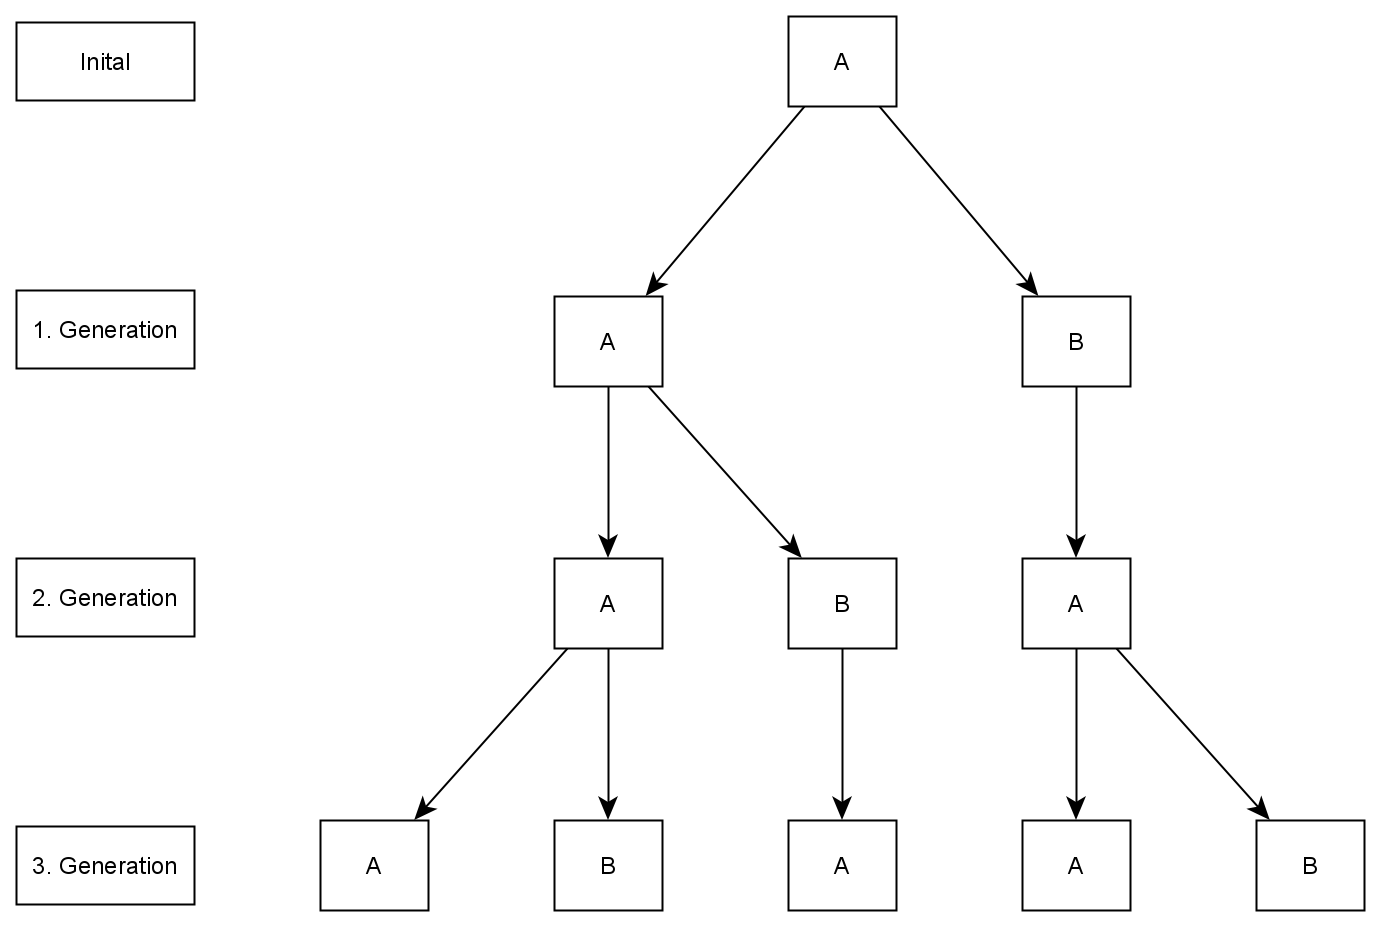
\includegraphics[width=0.7\columnwidth]{../graphs/Examples/simple_lsystem.png}
	\caption{Simple L-system}
	\label{figure:simple_lsystem}
\end{figure}

The first step is to use rule one, which replaces the nonterminal A with AB, resulting in the first generation. The result of the first generation ('AB') will be used to generate the second generation. For all nonterminals the productions will be parallel applied. In this case the nonterminals A and B will be replaced, because both have existing production rules. This results in the second generation with 'ABA' as result.

This process can be successively repeated recursive for a arbitrary amount of generations and create a fractal or plant with self-similar pieces. The more generations are calculated, the more detailed is the resulting state. 

\subsection{Grammar}
\label{section:grammar}
The definition of an L-system can be done similar to a Chomsky grammar, but there are some general differences. In Chomsky grammars the productions are applied sequentially, whereas in L-systems they can be applied parallel. This has some consequences for the formal properties of an L-system, for example a context-free L-system can produce a language which cannot be produced by a context-free Chomsky grammar.\footnote{Zitat abop vgl Seite 3  Abschnitt L-Systems}

\noindent This paper will only focus on a class of L-systems, the DOL-systems, which can be used for string based rewriting systems. This class is deterministic (D) and context-free (O) and can be formaly described  by a tuple:

\begin{center}
G = (V, $\omega$, P)
\end{center}

V: set of symbols as alphabet of the l-system - consiting of terminals and non terminals

$\omega$: axiom - nonempty word of the alphabet, which should contain at least one nonterminal

P: set of productions

\medskip
\noindent A production conistst of a predecessor, a nonterminal symbol of the alphabet, and a successor, the replacment of the nonterminal in the next generation.
To guarantee that the l-system is deterministic, there only can be one production for each nonterminal of the alphabet.The identity production is implicit a part of the set of productions.\footnote{Zitat vgl Seite 4 abop}

\medskip

If in the process of rewriting a terminal symbol is found, there will be no explicit production applied, but rather the identity production is applied. Terminals will therefore remain in future generations and won't extend an L-system with a production.

\medskip

\noindent As mentioned in section \ref{section:history} there are other extensions of a basic L-systems. The extensions introduce more possiblities for the generation process, like a non-deterministic behaviour. These extensions result in new grammars which can represent much complexer plants or fractals:

\begin{itemize}
\item Stochastic grammars: the system isn't deterministic anymore, because there can be multiple production rules for the same nonterminal with a probaility which results in a randomisation of the generation
\item Context senstive grammars: production not only look for the nonterminal, they rather look for the symbols bevor and after the current symbol to process, the context.
\item Parametric grammars: it is possible to set additional parameters for a symbol to influence the generation or the evaluation of the data
\end{itemize}

\subsection{Interpretation as turtle commands}
\label{section:turtle}
The L-systems introduced to this points are capable of creating a string based on a grammar. In order to create a graphic of a state of a L-system, the resulting state can be interpreted as commands of a turtle.

\noindent A turtle is a concept introduced by the language Logo as a tool for computer graphics.\footnote{Zitat VGL. Seite 179 Chappter 10 Logo book}

\noindent A state of a turtle can be described as a tuple\footnote{Zitat vgl abop Seite 6 ff}:

\begin{center}
S = (x,y, $\alpha$)
\end{center}

x and y are Cartesian coordinates

$\alpha$ is the direction in which a turtle is facing, called heading

\medskip

\noindent A turtle can move in the Cartesian coordinate system by altering the current state.You can think of it as a real turtle with a pen attached to it, walking on a paper. While moving in the coordinate system, or on the paper, the turtle can draw lines. Given this concept the turtle can receive different commands. The commands let the turtle walk on the paper or the coordinate system by altering the current state and drawing a line. For now I'll restrict this to a two dimensional coordinate system, but it is also possible to enhance it for a three dimensional coordinate system.

\medskip

\noindent The walking path of the turtle is controlled by commands. Therefor a defined step size \textit{d} and an angle \textit{$\theta$ } is needed to calculate the next state of the turtle.

\begin{itemize}
\item Draw: moves one step in the current facing direction drawing a line 
\item Move: moves one step in the current facing direction without drawing a line
\item Right-turn: turns to the right by the angle $\theta$
\item Left-turn: turns to the left by the angle $\theta$
\end{itemize}
\footnote{Zitat vlg cad book seitev 2 unteres drittel}

\noindent Additional to the state of the turtle the state there is a state for the pen. The pen state consist of the color and its width, which will result in more colorfull or different pictures.

\medskip

\noindent  With the given turtle concept is it possible to interpret the result of an L-system. Therefor a mapping between the symbols in the alphabet and the commands which should be called is needed.
This could be done by an arbitrary mapping between a nonterminal or a terminal and a command. For this paper the following mapping will be used, but the concept for the architecture includes the possibility to use other mappings in the future.

\noindent For the mapping alphabet V is used, which is a slightly extended version of the basic version of a L-system:

\begin{center}
V = (F, f, +, -, [,  ])
\end{center}

This alphabet will be mapped with extended turtle commands:

\begin{center}
\begin{tabular}{ c l }
Symbol & Turtle interpretation \\
\hline
F & Draw a line in the facing direction  \\ 
f & Move in the facing direction  \\  
+& Turn right  \\  
-& Turn left  \\  
{[} & save the current state in a stack  \\  
{]} & pop the last state form the stack and set it to the current state  \\

\end{tabular}
\end{center}

This interpretation enables to draw the result of the L-system by iterating over every terminal and nonterminal of the result state and calling the mapped command. If no command is mapped the symbol will be skipped.

\bigskip

STACK ENTFERENEN UND NUR SIMPLEN WEG NUTZEN

\bigskip

\subsection{Examples}
This section will present some examples for L-system grammars which create fractals. They use the introduced mapping of section \ref{section:turtle}.
  
\subsubsection{Koch curve}
This fractal will be generated with the simple axiom 'F' and just one production: F\rightarrow F+F--F+F 

\noindent The turtle will be initalized with an angle of 60° and an arbitrary length \textit{d} for a step.

\footnote{ADD A PICTURE and perhaps a source: http://mathforum.org/advanced/robertd/lsys2d.html}

\subsubsection{Sierpinski triangle}
This fractal will be created with 'F' as axiom and two productions:

\begin{itemize}
\item X\rightarrow YF+XF+Y
\item Y\rightarrow XF-YF-X
\end{itemize}

\noindent The turtle will be initalized with an angle of 60° and an arbitrary length \textit{d} for a step.
 
\footnote{ADD A PICTURE and SOURCE}


\pagebreak
\section{Architecture}
The primary goal of this paper is creating an architecture and an implementation of a L-system as described in section \ref{section:lindenmayer}. The focus of the architecture will be on flexibility and expandability and therefor is the following section splitted into several parts with discussions about different aspects of the final architecture.


\subsection{LSystem}
Core of the current architecture but still excahngable

What data to hold 
How to generate different generations (Suksessiver aufbau des L Systems)
 - why dont hold the generations - efficency
On the fly generation with an Output itertaor vs Graph

\subsection{Turtle}
Abstract interface with minimal set of needed functions

\subsection{Turtle command mapping}

\subsection{Configuration data}
convinient way of define a grammar - not hard coded - load form file


\section{LSystemHandler}

\begin{itemize}
	\item 
	\item Nutzung von beliebiger datenstruktur mit speziellen eigenschaften -> Semantische Schnittstelle
	\item Bekommt die Daten aus dem FileHandler, kann aber aus allem kommen - belieib in andere Sachen einbindbar
\end{itemize}

\section{LSystem Datastructure}

\begin{itemize}
	\item Tree like sturcture
	\item save data not double only save pointers to the data
	\item provides access to the data with an iterator
\end{itemize}

\section{Parser for the lsystem}
\begin{itemize}
	\item Parses the result of the l system
	\item calls the Turtle Graphic on the fly
	
	\item Problem for now -> not very flexible (perhaps for the future: provide which function to call for which object)
\end{itemize}


\section{Implementation}
\subsection{Build System}
\label{section:buildsystem}
The first important point 

\begin{itemize}
	\item Cmake as buildsystem
	\item reasons why cmake
	\item problems ?
\end{itemize}


\subsection{TurtleGraphic}
\subsubsection{TestTurtle}
\subsubsection{CairoTurtle}
\subsubsection{Further implementations}
SVG implementation


\section{Tests}
\section{Examples}
\section{Problems and Restrictions}
\section{Outlook}
\footnote{\fullcite{prusinkiewiczp.lindenmayera.2004}}
\end{document}